\documentclass{beamer}

%--------------beamer---------------
\usetheme{Warsaw}
\usecolortheme{wolverine}
\usefonttheme{serif}
\usepackage{tikz}
\useinnertheme{rectangles}
\useoutertheme{miniframes}
\setbeamercolor*{mini frame}{fg=black,bg=white}
\setbeamercolor{section in head/foot}{fg=black, bg=yellow}

%-------------packages--------------
\usepackage{helvet} %font package
\usepackage{graphicx} % Required for inserting images
\graphicspath{ {./images/} }
\usepackage{amsmath}
% Code syntax highlighter
\usepackage{minted}
\setbeamertemplate{caption}{\raggedright\insertcaption\par}

\definecolor{col_block_title}{HTML}{2a9d8f}
\setbeamercolor{block title}{bg=col_block_title}

\definecolor{col_block_body}{HTML}{f1faee}
\setbeamercolor{block body}{bg=col_block_body}

\definecolor{col_example_title}{HTML}{f18701}
\setbeamercolor{block title example}{bg=col_example_title}

\definecolor{col_example_body}{HTML}{FBF7F4}
\setbeamercolor{block body example}{bg=col_example_body}

\definecolor{col_alert_title}{HTML}{f72585}
\setbeamercolor{block title alerted}{bg=col_alert_title}

\definecolor{col_alert_body}{HTML}{FBF7F4}
\setbeamercolor{block body alerted}{bg=col_alert_body}

%------------title page-------------

\addtobeamertemplate{navigation symbols}{}{%
    \usebeamerfont{footline}%
    \usebeamercolor[fg]{footline}%
    \hspace{1em}%
    \insertframenumber/\inserttotalframenumber
}
\title{Segment Tree}
\author[Sadat (1905001) Asif (1905004)]
{Mohammad Sadat Hossain\inst{1} \and Asif Azad\inst{2}}
\institute[VFU] % (optional)
{
  \inst{1}1905001
  \and
  \inst{2}1905004
  \and
  \inst{1,2}Department of Computer Science and Technology, BUET
}

%-------------main document--------------
\setbeamertemplate{blocks}[rounded][shadow=true]
\begin{document}

\begin{frame}
    \titlepage
\end{frame}

\tikzstyle{visible_node} = [rectangle, rounded corners, draw=blue, thick, fill=blue!10, text width=15pt, text=black, text centered]

\section{Introduction}
\begin{frame}{The Problem}
    \begin{block}{Range Sum Query}
     You are given an integer array $a$. Answer $q$ queries of the following form: \\
     \centering
     \begin{itemize}
     \item $sum(i, j)$ : returns $\sum_{k=i}^{j} a[k]$
     \end{itemize}
    \end{block}
    \pause
    \begin{example}
    \centering
        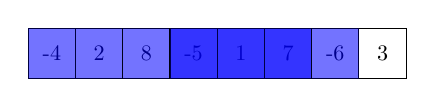
\begin{tikzpicture}[scale=0.8,transform shape]
        \onslide <2->
        \foreach \i/\j in {1/-4,2/2,3/8,4/-5,5/1,6/7,7/-6,8/3} {
            \pgfmathsetmacro\result{\i-1}
            \node[draw,rectangle, minimum width=0.75cm, minimum height=0.8cm] at (\result * 0.75,0) {\j};
        };
        \onslide <3>
        \foreach \i in {1,2,3,4,5,6} {
            \pgfmathsetmacro\result{\i-1}
            \node[draw, rectangle, minimum width=0.75cm, opacity=0.55, fill=blue, minimum height=0.8cm] at (\result * 0.75, 0){};
        };
        \onslide <4>
        \foreach \i in {4,5,6,7} {
            \pgfmathsetmacro\result{\i-1}
            \node[draw, rectangle, minimum width=0.75cm, opacity=0.55, fill=blue, minimum height=0.8cm] at (\result * 0.75, 0){};
        };
        \end{tikzpicture}
        \onslide<3-> {$sum(0, 5) = -4 + 2 + 8 + (-5) + 1 + 7 = 9$}
        \onslide<4-> {$sum(3, 6) = -5 + 1 + 7 + (-6) = -3$}

    \end{example}
\end{frame}

\begin{frame}{Solution Ideas}
		\tikzstyle{textbox} = [rectangle, draw=white, fill=blue!0]
		\begin{itemize}
			\onslide<2->{\item \textbf{Naive Solution} : An $O(n)$ loop for each query.}
			\onslide<3->{\item \textbf{Smart Solution} : Precompute prefix sums, then answer the queries in $O(1)$.}
		\end{itemize}
		\onslide<4->
		\begin{example}
			\centering
			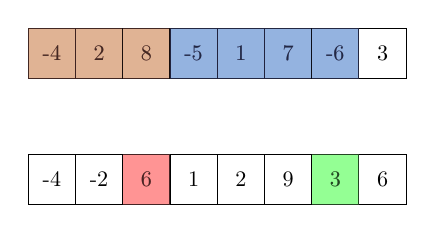
\begin{tikzpicture}[scale=0.8,transform shape]
				\onslide <4->
				\foreach \i/\j in {1/-4,2/2,3/8,4/-5,5/1,6/7,7/-6,8/3} {
					\pgfmathsetmacro\result{\i-1}
					\node[draw,rectangle, minimum width=0.75cm, minimum height=0.8cm] at (\result * 0.75,2) {\j};
				};
                \onslide <5->
				\foreach \i/\j in {1/-4,2/-2,3/6,4/1,5/2,6/9,7/3,8/6} {
					\pgfmathsetmacro\result{\i-1}
					\node[draw,rectangle, minimum width=0.75cm, minimum height=0.8cm] at (\result * 0.75,0) {\j};
				};
				\onslide <6>
                % main array
    				\foreach \i/\j in {1/-4,2/2,3/8,4/-5,5/1,6/7,7/-6} {
    					\pgfmathsetmacro\result{\i-1}
    					\node[draw, rectangle, minimum width=0.75cm, opacity=0.6, fill=green!50, minimum height=0.8cm, text=black] at (\result * 0.75, 2){\j};
    				};
                % prefix sum array
                \onslide <6>
                    \foreach \i/\j in {7/3} {
                        \pgfmathsetmacro\result{\i-1}
                        \node[draw, rectangle, minimum width=0.75cm, opacity=0.6, fill=green!50, minimum height=0.8cm, text=black] at (\result * 0.75,0) {\j};
                    };
				\onslide <7> 
                % main array
    				\foreach \i/\j in {1/-4,2/2,3/8} {
    					\pgfmathsetmacro\result{\i-1}
    					\node[draw, rectangle, minimum width=0.75cm, opacity=0.6, fill=red!50, minimum height=0.8cm] at (\result * 0.75, 2){\j};
    				};
                \onslide <7>
                % prefix sum array
                    \foreach \i/\j in {3/6} {
                        \pgfmathsetmacro\result{\i-1}
                        \node[draw, rectangle, minimum width=0.75cm, opacity=0.6, fill=red!50, minimum height=0.8cm] at (\result * 0.75,0) {\j};
                    };
            \onslide <8> 
                % main array
    				\foreach \i/\j in {4/-5,5/1,6/7,7/-6} {
    					\pgfmathsetmacro\result{\i-1}
    					\node[draw, rectangle, minimum width=0.75cm, opacity=0.6, fill=blue!50, minimum height=0.8cm] at (\result * 0.75, 2){\j};
    				};
                \onslide <8>
                % prefix sum array
                    \foreach \i/\j in {3/6} {
                        \pgfmathsetmacro\result{\i-1}
                        \node[draw, rectangle, minimum width=0.75cm, opacity=0.6, fill=red!50, minimum height=0.8cm] at (\result * 0.75,0) {\j};
                    };
                \onslide<8>
                \foreach \i/\j in {7/3} {
                        \pgfmathsetmacro\result{\i-1}
                        \node[draw, rectangle, minimum width=0.75cm, opacity=0.6, fill=green!50, minimum height=0.8cm, text=black] at (\result * 0.75,0) {\j};
                    };
			\end{tikzpicture}
			\onslide<8> {$sum(3, 6) = sum(0, 6) - sum(0, 2) = 3 - 6 = -3$}
			
		\end{example}
	\end{frame}

\begin{frame}{}
    \begin{center}
    \begin{columns}
    \column{0.5\textwidth}
    \onslide<1->{\centering{ \textbf{\textcolor{black}{That was easy!}}\\
    
\includegraphics[width=40mm, height=50mm]{seg-meme1.jpg}}}

    \column{0.5\textwidth}
    \onslide<2->{\centering{\textbf{\textcolor{black}{Let's see a hard version}}\\
    
\includegraphics[width=40mm, height=50mm]{seg-meme2.jpg}}}

    \end{columns}
\end{center}
\end{frame}

\begin{frame}{A More Challenging Problem}
    \begin{block}{Range Sum Query}
     You are given an integer array $a$. Answer $q$ queries of the following form: \\
     \centering
     \begin{itemize}
     \item $sum(i, j)$ : returns $\sum_{k=i}^{j} a[k]$
     \pause
     \item $update(i, v)$ : do $a[i] = v$
     \end{itemize}
    \end{block}
    \pause
    \begin{alertblock}{Will Prefix Sum Work Well Now?}
    \pause
    No, update makes it $O(n)$. Look for something better!
    \end{alertblock}
\end{frame}

\section{Tree Construction}
%%segment tree node styles
\tikzstyle{node_partially_contained} = [draw=black, fill=yellow]
\tikzstyle{node_fully_contained} = [draw=green, fill=green!20]
\tikzstyle{node_not_contained} = [draw=red, fill=red!10]
\tikzstyle{invisible} = [draw=white, fill=white, text=white, text width=15pt]
\tikzstyle{every node} = [rectangle, rounded corners, draw=blue, thick, fill=blue!10, text width=15pt, text centered]
\tikzstyle{level 1} = [sibling distance=50mm]
\tikzstyle{level 2} = [sibling distance=25mm]
\tikzstyle{level 3} = [sibling distance=12mm]
\tikzstyle{visible_edge} = [->, draw, blue, thick]
\tikzstyle{edge from parent} = [->,draw, blue, thick]

%% build_frame_1
\begin{frame}[c]{Construction of Segment Tree}

    \centering
    \begin{tikzpicture}
        \tikzstyle{every node} = [invisible]
        \tikzstyle{edge from parent} = [invisible]
        \path
        node[label=right:\text{a[0\ldots7]}]{6}
        child{
                node[label=right:\text{a[0\ldots3]}]{1}
                child{
                        node[label=right:\text{a[0\ldots1]}]{-2}
                        child{
                                node[label={[text=black]below:\text{a[0]}}, visible_node]{-4}
                            }
                        child{
                                node[label={[text=black]below:\text{a[1]}}, visible_node]{2}
                            }
                    }
                child{
                        node[label=right:\text{a[2\ldots3]}]{3}
                        child{
                                node[label={[text=black]below:\text{a[2]}}, visible_node]{8}
                            }
                        child{
                                node[label={[text=black]below:\text{a[3]}}, visible_node]{-5}
                            }
                    }
            }
        child{
                node[label=right:\text{a[4\ldots7]}]{5}
                child{
                        node[label=right:\text{a[4\ldots5]}]{8}
                        child{
                                node[label={[text=black]below:\text{a[4]}}, visible_node]{1}
                            }
                        child{
                                node[label={[text=black]below:\text{a[5]}}, visible_node]{7}
                            }
                    }
                child{
                        node[label=right:\text{a[6\ldots7]}]{-3}
                        child{
                                node[label={[text=black]below:\text{a[6]}}, visible_node]{-6}
                            }
                        child{
                                node[label={[text=black]below:\text{a[7]}}, visible_node]{3}
                            }
                    }
            }
        ;

    \end{tikzpicture}

\end{frame}

%% build_frame_2
\begin{frame}[c]{Construction of Segment Tree}

    \centering
    \begin{tikzpicture}
        \tikzstyle{every node} = [invisible]
        \tikzstyle{edge from parent} = [invisible]
        \path
        node[label=right:\text{a[0\ldots7]}]{6}
        child{
                node[label=right:\text{a[0\ldots3]}]{1}
                child{
                        node[label={[text=black]right:\text{a[0\ldots1]}}, visible_node]{-2}
                        child{
                                node[label={[text=black]below:\text{a[0]}}, visible_node]{-4} edge from parent[visible_edge]
                            }
                        child{
                                node[label={[text=black]below:\text{a[1]}}, visible_node]{2} edge from parent[visible_edge]
                            }
                    }
                child{
                        node[label={[text=black]right:\text{a[2\ldots3]}}, visible_node]{3}
                        child{
                                node[label={[text=black]below:\text{a[2]}}, visible_node]{8} edge from parent[visible_edge]
                            }
                        child{
                                node[label={[text=black]below:\text{a[3]}}, visible_node]{-5} edge from parent[visible_edge]
                            }
                    }
            }
        child{
                node[label=right:\text{a[4\ldots7]}]{5}
                child{
                        node[label={[text=black]right:\text{a[4\ldots5]}}, visible_node]{8}
                        child{
                                node[label={[text=black]below:\text{a[4]}}, visible_node]{1} edge from parent[visible_edge]
                            }
                        child{
                                node[label={[text=black]below:\text{a[5]}}, visible_node]{7} edge from parent[visible_edge]
                            }
                    }
                child{
                        node[label={[text=black]right:\text{a[6\ldots7]}}, visible_node]{-3}
                        child{
                                node[label={[text=black]below:\text{a[6]}}, visible_node]{-6} edge from parent[visible_edge]
                            }
                        child{
                                node[label={[text=black]below:\text{a[7]}}, visible_node]{3} edge from parent[visible_edge]
                            }
                    }
            }
        ;

    \end{tikzpicture}

\end{frame}

%% build_frame_3
\begin{frame}[c]{Construction of Segment Tree}

    \centering
    \begin{tikzpicture}
        \tikzstyle{every node} = [invisible]
        \tikzstyle{edge from parent} = [invisible]
        \path
        node[label=right:\text{a[0\ldots7]}]{6}
        child{
                node[label={[text=black]right:\text{a[0\ldots3]}}, visible_node]{1}
                child{
                        node[label={[text=black]right:\text{a[0\ldots1]}}, visible_node]{-2} edge from parent[visible_edge]
                        child{
                                node[label={[text=black]below:\text{a[0]}}, visible_node]{-4} edge from parent[visible_edge]
                            }
                        child{
                                node[label={[text=black]below:\text{a[1]}}, visible_node]{2} edge from parent[visible_edge]
                            }
                    }
                child{
                        node[label={[text=black]right:\text{a[2\ldots3]}}, visible_node]{3} edge from parent[visible_edge]
                        child{
                                node[label={[text=black]below:\text{a[2]}}, visible_node]{8} edge from parent[visible_edge]
                            }
                        child{
                                node[label={[text=black]below:\text{a[3]}}, visible_node]{-5} edge from parent[visible_edge]
                            }
                    }
            }
        child{
                node[label={[text=black]right:\text{a[4\ldots7]}}, visible_node]{5}
                child{
                        node[label={[text=black]right:\text{a[4\ldots5]}}, visible_node]{8} edge from parent[visible_edge]
                        child{
                                node[label={[text=black]below:\text{a[4]}}, visible_node]{1} edge from parent[visible_edge]
                            }
                        child{
                                node[label={[text=black]below:\text{a[5]}}, visible_node]{7} edge from parent[visible_edge]
                            }
                    }
                child{
                        node[label={[text=black]right:\text{a[6\ldots7]}}, visible_node]{-3} edge from parent[visible_edge]
                        child{
                                node[label={[text=black]below:\text{a[6]}}, visible_node]{-6} edge from parent[visible_edge]
                            }
                        child{
                                node[label={[text=black]below:\text{a[7]}}, visible_node]{3} edge from parent[visible_edge]
                            }
                    }
            }
        ;

    \end{tikzpicture}

\end{frame}

%% build_frame_4
\begin{frame}[c]{Construction of Segment Tree}

    \centering
    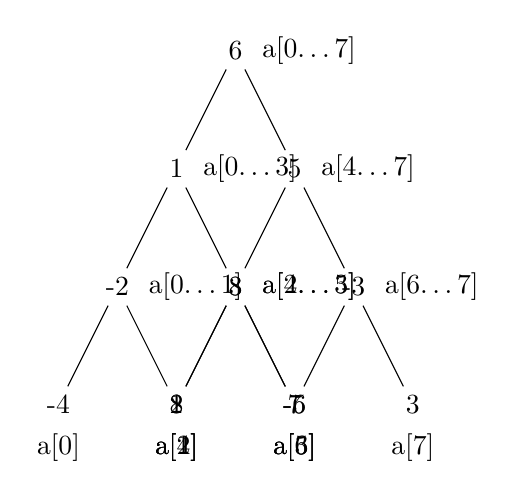
\begin{tikzpicture}
        \path
        node[label=right:\text{a[0\ldots7]}]{6}
        child{
                node[label=right:\text{a[0\ldots3]}]{1}
                child{
                        node[label=right:\text{a[0\ldots1]}]{-2}
                        child{
                                node[label=below:\text{a[0]}]{-4}
                            }
                        child{
                                node[label=below:\text{a[1]}]{2}
                            }
                    }
                child{
                        node[label=right:\text{a[2\ldots3]}]{3}
                        child{
                                node[label=below:\text{a[2]}]{8}
                            }
                        child{
                                node[label=below:\text{a[3]}]{-5}
                            }
                    }
            }
        child{
                node[label=right:\text{a[4\ldots7]}]{5}
                child{
                        node[label=right:\text{a[4\ldots5]}]{8}
                        child{
                                node[label=below:\text{a[4]}]{1}
                            }
                        child{
                                node[label=below:\text{a[5]}]{7}
                            }
                    }
                child{
                        node[label=right:\text{a[6\ldots7]}]{-3}
                        child{
                                node[label=below:\text{a[6]}]{-6}
                            }
                        child{
                                node[label=below:\text{a[7]}]{3}
                            }
                    }
            }
        ;

    \end{tikzpicture}
\end{frame}
\begin{frame}[fragile]
    \frametitle{Build Code}
    \scriptsize
    \begin{minted}[frame=lines, framesep=2mm, baselinestretch=1.2,fontsize=\footnotesize, autogobble, obeytabs=true, tabsize=3]{cpp}
        void build(int arr[], int idx, int l, int r) {
            if (l == r) tree[idx] = arr[l];
            else {
                int mid = (l + r) / 2;
                build(arr, idx * 2, l, mid);
                build(arr, idx * 2 + 1, mid + 1, r);
                tree[idx] = tree[idx * 2] + tree[idx * 2 + 1];
            }
        }
    \end{minted}
\end{frame}

\section{Update Query}
%% update_frame_1
\begin{frame}[c]{Update Segment Tree}

    \centering
    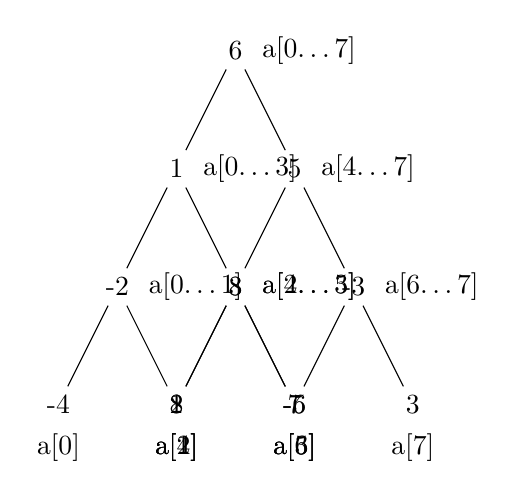
\begin{tikzpicture}
        \path
        node[label=right:\text{a[0\ldots7]}]{6}
        child{
                node[label=right:\text{a[0\ldots3]}]{1}
                child{
                        node[label=right:\text{a[0\ldots1]}]{-2}
                        child{
                                node[label=below:\text{a[0]}]{-4}
                            }
                        child{
                                node[label=below:\text{a[1]}]{2}
                            }
                    }
                child{
                        node[label=right:\text{a[2\ldots3]}]{3}
                        child{
                                node[label=below:\text{a[2]}]{8}
                            }
                        child{
                                node[label=below:\text{a[3]}]{-5}
                            }
                    }
            }
        child{
                node[label=right:\text{a[4\ldots7]}]{5}
                child{
                        node[label=right:\text{a[4\ldots5]}]{8}
                        child{
                                node[label=below:\text{a[4]}]{1}
                            }
                        child{
                                node[label=below:\text{a[5]}]{7}
                            }
                    }
                child{
                        node[label=right:\text{a[6\ldots7]}]{-3}
                        child{
                                node[label=below:\text{a[6]}]{-6}
                            }
                        child{
                                node[label=below:\text{a[7]}]{3}
                            }
                    }
            }
        ;

    \end{tikzpicture}

    $update(2, -7):a[2] = -7$
\end{frame}

%% update_frame_2
\begin{frame}[c]{Update Segment Tree}

    \centering
    \begin{tikzpicture}
        \path
        node[label=right:\text{a[0\ldots7]}, node_partially_contained]{6}
        child{
                node[label=right:\text{a[0\ldots3]}]{1}
                child{
                        node[label=right:\text{a[0\ldots1]}]{-2}
                        child{
                                node[label=below:\text{a[0]}]{-4}
                            }
                        child{
                                node[label=below:\text{a[1]}]{2}
                            }
                    }
                child{
                        node[label=right:\text{a[2\ldots3]}]{3}
                        child{
                                node[label=below:\text{a[2]}]{8}
                            }
                        child{
                                node[label=below:\text{a[3]}]{-5}
                            }
                    }
            }
        child{
                node[label=right:\text{a[4\ldots7]}]{5}
                child{
                        node[label=right:\text{a[4\ldots5]}]{8}
                        child{
                                node[label=below:\text{a[4]}]{1}
                            }
                        child{
                                node[label=below:\text{a[5]}]{7}
                            }
                    }
                child{
                        node[label=right:\text{a[6\ldots7]}]{-3}
                        child{
                                node[label=below:\text{a[6]}]{-6}
                            }
                        child{
                                node[label=below:\text{a[7]}]{3}
                            }
                    }
            }
        ;

    \end{tikzpicture}

    $update(2, -7):a[2] = -7$
\end{frame}

%% update_frame_3
\begin{frame}[c]{Update Segment Tree}

    \centering
    \begin{tikzpicture}
        \path
        node[label=right:\text{a[0\ldots7]}, node_partially_contained]{6}
        child{
                node[label=right:\text{a[0\ldots3]}, node_partially_contained]{1}
                child{
                        node[label=right:\text{a[0\ldots1]}]{-2}
                        child{
                                node[label=below:\text{a[0]}]{-4}
                            }
                        child{
                                node[label=below:\text{a[1]}]{2}
                            }
                    }
                child{
                        node[label=right:\text{a[2\ldots3]}]{3}
                        child{
                                node[label=below:\text{a[2]}]{8}
                            }
                        child{
                                node[label=below:\text{a[3]}]{-5}
                            }
                    }
            }
        child{
                node[label=right:\text{a[4\ldots7]}]{5}
                child{
                        node[label=right:\text{a[4\ldots5]}]{8}
                        child{
                                node[label=below:\text{a[4]}]{1}
                            }
                        child{
                                node[label=below:\text{a[5]}]{7}
                            }
                    }
                child{
                        node[label=right:\text{a[6\ldots7]}]{-3}
                        child{
                                node[label=below:\text{a[6]}]{-6}
                            }
                        child{
                                node[label=below:\text{a[7]}]{3}
                            }
                    }
            }
        ;

    \end{tikzpicture}

    $update(2, -7):a[2] = -7$
\end{frame}

%% update_frame_4
\begin{frame}[c]{Update Segment Tree}

    \centering
    \begin{tikzpicture}
        \path
        node[label=right:\text{a[0\ldots7]}, node_partially_contained]{6}
        child{
                node[label=right:\text{a[0\ldots3]}, node_partially_contained]{1}
                child{
                        node[label=right:\text{a[0\ldots1]}]{-2}
                        child{
                                node[label=below:\text{a[0]}]{-4}
                            }
                        child{
                                node[label=below:\text{a[1]}]{2}
                            }
                    }
                child{
                        node[label=right:\text{a[2\ldots3]}, node_partially_contained]{3}
                        child{
                                node[label=below:\text{a[2]}]{8}
                            }
                        child{
                                node[label=below:\text{a[3]}]{-5}
                            }
                    }
            }
        child{
                node[label=right:\text{a[4\ldots7]}]{5}
                child{
                        node[label=right:\text{a[4\ldots5]}]{8}
                        child{
                                node[label=below:\text{a[4]}]{1}
                            }
                        child{
                                node[label=below:\text{a[5]}]{7}
                            }
                    }
                child{
                        node[label=right:\text{a[6\ldots7]}]{-3}
                        child{
                                node[label=below:\text{a[6]}]{-6}
                            }
                        child{
                                node[label=below:\text{a[7]}]{3}
                            }
                    }
            }
        ;

    \end{tikzpicture}

    $update(2, -7):a[2] = -7$
\end{frame}

%% update_frame_5
\begin{frame}[c]{Update Segment Tree}

    \centering
    \begin{tikzpicture}
        \path
        node[label=right:\text{a[0\ldots7]}, node_partially_contained]{6}
        child{
                node[label=right:\text{a[0\ldots3]}, node_partially_contained]{1}
                child{
                        node[label=right:\text{a[0\ldots1]}]{-2}
                        child{
                                node[label=below:\text{a[0]}]{-4}
                            }
                        child{
                                node[label=below:\text{a[1]}]{2}
                            }
                    }
                child{
                        node[label=right:\text{a[2\ldots3]}, node_partially_contained]{3}
                        child{
                                node[label=below:\text{a[2]}, node_partially_contained]{8}
                            }
                        child{
                                node[label=below:\text{a[3]}]{-5}
                            }
                    }
            }
        child{
                node[label=right:\text{a[4\ldots7]}]{5}
                child{
                        node[label=right:\text{a[4\ldots5]}]{8}
                        child{
                                node[label=below:\text{a[4]}]{1}
                            }
                        child{
                                node[label=below:\text{a[5]}]{7}
                            }
                    }
                child{
                        node[label=right:\text{a[6\ldots7]}]{-3}
                        child{
                                node[label=below:\text{a[6]}]{-6}
                            }
                        child{
                                node[label=below:\text{a[7]}]{3}
                            }
                    }
            }
        ;

    \end{tikzpicture}

    $update(2, -7):a[2] = -7$
\end{frame}

%% update_frame_6
\begin{frame}[c]{Update Segment Tree}

    \centering
    \begin{tikzpicture}
        \path
        node[label=right:\text{a[0\ldots7]}, node_partially_contained]{6}
        child{
                node[label=right:\text{a[0\ldots3]}, node_partially_contained]{1}
                child{
                        node[label=right:\text{a[0\ldots1]}]{-2}
                        child{
                                node[label=below:\text{a[0]}]{-4}
                            }
                        child{
                                node[label=below:\text{a[1]}]{2}
                            }
                    }
                child{
                        node[label=right:\text{a[2\ldots3]}, node_partially_contained]{3}
                        child{
                                node[label=below:\text{a[2]}, node_fully_contained]{-7}
                            }
                        child{
                                node[label=below:\text{a[3]}]{-5}
                            }
                    }
            }
        child{
                node[label=right:\text{a[4\ldots7]}]{5}
                child{
                        node[label=right:\text{a[4\ldots5]}]{8}
                        child{
                                node[label=below:\text{a[4]}]{1}
                            }
                        child{
                                node[label=below:\text{a[5]}]{7}
                            }
                    }
                child{
                        node[label=right:\text{a[6\ldots7]}]{-3}
                        child{
                                node[label=below:\text{a[6]}]{-6}
                            }
                        child{
                                node[label=below:\text{a[7]}]{3}
                            }
                    }
            }
        ;

    \end{tikzpicture}

    $update(2, -7):a[2] = -7$
\end{frame}

%% update_frame_7
\begin{frame}[c]{Update Segment Tree}

    \centering
    \begin{tikzpicture}
        \path
        node[label=right:\text{a[0\ldots7]}, node_partially_contained]{6}
        child{
                node[label=right:\text{a[0\ldots3]}, node_partially_contained]{1}
                child{
                        node[label=right:\text{a[0\ldots1]}]{-2}
                        child{
                                node[label=below:\text{a[0]}]{-4}
                            }
                        child{
                                node[label=below:\text{a[1]}]{2}
                            }
                    }
                child{
                        node[label=right:\text{a[2\ldots3]}, node_fully_contained]{-12}
                        child{
                                node[label=below:\text{a[2]}, node_fully_contained]{-7}
                            }
                        child{
                                node[label=below:\text{a[3]}]{-5}
                            }
                    }
            }
        child{
                node[label=right:\text{a[4\ldots7]}]{5}
                child{
                        node[label=right:\text{a[4\ldots5]}]{8}
                        child{
                                node[label=below:\text{a[4]}]{1}
                            }
                        child{
                                node[label=below:\text{a[5]}]{7}
                            }
                    }
                child{
                        node[label=right:\text{a[6\ldots7]}]{-3}
                        child{
                                node[label=below:\text{a[6]}]{-6}
                            }
                        child{
                                node[label=below:\text{a[7]}]{3}
                            }
                    }
            }
        ;

    \end{tikzpicture}

    $update(2, -7):a[2] = -7$
\end{frame}

%% update_frame_8
\begin{frame}[c]{Update Segment Tree}

    \centering
    \begin{tikzpicture}
        \path
        node[label=right:\text{a[0\ldots7]}, node_partially_contained]{6}
        child{
                node[label=right:\text{a[0\ldots3]}, node_fully_contained]{-14}
                child{
                        node[label=right:\text{a[0\ldots1]}]{-2}
                        child{
                                node[label=below:\text{a[0]}]{-4}
                            }
                        child{
                                node[label=below:\text{a[1]}]{2}
                            }
                    }
                child{
                        node[label=right:\text{a[2\ldots3]}, node_fully_contained]{-12}
                        child{
                                node[label=below:\text{a[2]}, node_fully_contained]{-7}
                            }
                        child{
                                node[label=below:\text{a[3]}]{-5}
                            }
                    }
            }
        child{
                node[label=right:\text{a[4\ldots7]}]{5}
                child{
                        node[label=right:\text{a[4\ldots5]}]{8}
                        child{
                                node[label=below:\text{a[4]}]{1}
                            }
                        child{
                                node[label=below:\text{a[5]}]{7}
                            }
                    }
                child{
                        node[label=right:\text{a[6\ldots7]}]{-3}
                        child{
                                node[label=below:\text{a[6]}]{-6}
                            }
                        child{
                                node[label=below:\text{a[7]}]{3}
                            }
                    }
            }
        ;

    \end{tikzpicture}

    $update(2, -7):a[2] = -7$
\end{frame}

%% update_frame_9
\begin{frame}[c]{Update Segment Tree}

    \centering
    \begin{tikzpicture}
        \path
        node[label=right:\text{a[0\ldots7]}, node_fully_contained]{-9}
        child{
                node[label=right:\text{a[0\ldots3]}, node_fully_contained]{-14}
                child{
                        node[label=right:\text{a[0\ldots1]}]{-2}
                        child{
                                node[label=below:\text{a[0]}]{-4}
                            }
                        child{
                                node[label=below:\text{a[1]}]{2}
                            }
                    }
                child{
                        node[label=right:\text{a[2\ldots3]}, node_fully_contained]{-12}
                        child{
                                node[label=below:\text{a[2]}, node_fully_contained]{-7}
                            }
                        child{
                                node[label=below:\text{a[3]}]{-5}
                            }
                    }
            }
        child{
                node[label=right:\text{a[4\ldots7]}]{5}
                child{
                        node[label=right:\text{a[4\ldots5]}]{8}
                        child{
                                node[label=below:\text{a[4]}]{1}
                            }
                        child{
                                node[label=below:\text{a[5]}]{7}
                            }
                    }
                child{
                        node[label=right:\text{a[6\ldots7]}]{-3}
                        child{
                                node[label=below:\text{a[6]}]{-6}
                            }
                        child{
                                node[label=below:\text{a[7]}]{3}
                            }
                    }
            }
        ;

    \end{tikzpicture}

    $update(2, -7):a[2] = -7$
\end{frame}

\begin{frame}[fragile]
		\frametitle{Update Code}
		\scriptsize
		\begin{minted}[frame=lines, framesep=2mm, baselinestretch=1.2,fontsize=\footnotesize, autogobble, obeytabs=true,tabsize=3]{cpp}
        void update(int idx, int l, int r, int pos, int new_val) {
            if (l == r) 
                tree[idx] = new_val;
            else {
                int mid = (l + r) / 2;
                if (pos <= mid) 
                   update(idx * 2, l, mid, pos, new_val);
                else 
                   update(idx * 2 + 1, mid + 1, r, pos, new_val);
                tree[idx] = tree[idx * 2] + tree[idx * 2 + 1];
            }
        }
		\end{minted}
	\end{frame}

\section{Query on Tree}
%% query_frame_1
\begin{frame}[c]{Answering Query From Segment Tree}

    \centering
    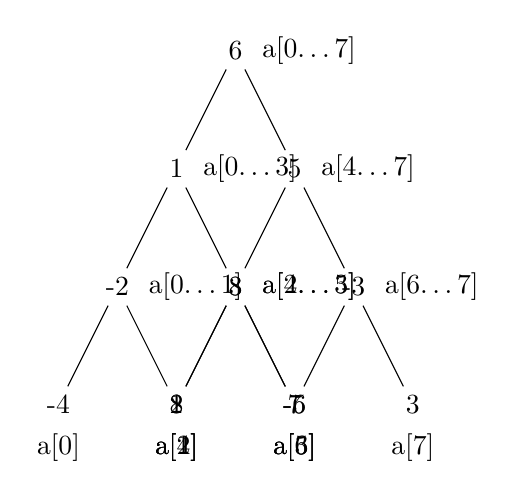
\begin{tikzpicture}
        \path
        node[label=right:\text{a[0\ldots7]}]{6}
        child{
                node[label=right:\text{a[0\ldots3]}]{1}
                child{
                        node[label=right:\text{a[0\ldots1]}]{-2}
                        child{
                                node[label=below:\text{a[0]}]{-4}
                            }
                        child{
                                node[label=below:\text{a[1]}]{2}
                            }
                    }
                child{
                        node[label=right:\text{a[2\ldots3]}]{3}
                        child{
                                node[label=below:\text{a[2]}]{8}
                            }
                        child{
                                node[label=below:\text{a[3]}]{-5}
                            }
                    }
            }
        child{
                node[label=right:\text{a[4\ldots7]}]{5}
                child{
                        node[label=right:\text{a[4\ldots5]}]{8}
                        child{
                                node[label=below:\text{a[4]}]{1}
                            }
                        child{
                                node[label=below:\text{a[5]}]{7}
                            }
                    }
                child{
                        node[label=right:\text{a[6\ldots7]}]{-3}
                        child{
                                node[label=below:\text{a[6]}]{-6}
                            }
                        child{
                                node[label=below:\text{a[7]}]{3}
                            }
                    }
            }
        ;
    \end{tikzpicture}
    \vfill
    $sum(0, 5) = ?$
\end{frame}

%% query_frame_2
\begin{frame}[c]{Answering Query From Segment Tree}

    \centering
    \begin{tikzpicture}
        \path
        node[label=right:\text{a[0\ldots7]}, node_partially_contained]{6}
        child{
                node[label=right:\text{a[0\ldots3]}]{1}
                child{
                        node[label=right:\text{a[0\ldots1]}]{-2}
                        child{
                                node[label=below:\text{a[0]}]{-4}
                            }
                        child{
                                node[label=below:\text{a[1]}]{2}
                            }
                    }
                child{
                        node[label=right:\text{a[2\ldots3]}]{3}
                        child{
                                node[label=below:\text{a[2]}]{8}
                            }
                        child{
                                node[label=below:\text{a[3]}]{-5}
                            }
                    }
            }
        child{
                node[label=right:\text{a[4\ldots7]}]{5}
                child{
                        node[label=right:\text{a[4\ldots5]}]{8}
                        child{
                                node[label=below:\text{a[4]}]{1}
                            }
                        child{
                                node[label=below:\text{a[5]}]{7}
                            }
                    }
                child{
                        node[label=right:\text{a[6\ldots7]}]{-3}
                        child{
                                node[label=below:\text{a[6]}]{-6}
                            }
                        child{
                                node[label=below:\text{a[7]}]{3}
                            }
                    }
            }
        ;

    \end{tikzpicture}
    \vfill
    $sum(0, 5) = ?$
\end{frame}

%% query_frame_3
\begin{frame}[c]{Answering Query From Segment Tree}

    \centering
    \begin{tikzpicture}
        \path
        node[label=right:\text{a[0\ldots7]}, node_partially_contained]{6}
        child{
                node[label=right:\text{a[0\ldots3]}, node_partially_contained]{1}
                child{
                        node[label=right:\text{a[0\ldots1]}]{-2}
                        child{
                                node[label=below:\text{a[0]}]{-4}
                            }
                        child{
                                node[label=below:\text{a[1]}]{2}
                            }
                    }
                child{
                        node[label=right:\text{a[2\ldots3]}]{3}
                        child{
                                node[label=below:\text{a[2]}]{8}
                            }
                        child{
                                node[label=below:\text{a[3]}]{-5}
                            }
                    }
            }
        child{
                node[label=right:\text{a[4\ldots7]}, node_partially_contained]{5}
                child{
                        node[label=right:\text{a[4\ldots5]}]{8}
                        child{
                                node[label=below:\text{a[4]}]{1}
                            }
                        child{
                                node[label=below:\text{a[5]}]{7}
                            }
                    }
                child{
                        node[label=right:\text{a[6\ldots7]}]{-3}
                        child{
                                node[label=below:\text{a[6]}]{-6}
                            }
                        child{
                                node[label=below:\text{a[7]}]{3}
                            }
                    }
            }
        ;

    \end{tikzpicture}
    \vfill
    $sum(0, 5) = ?$
\end{frame}

%% query_frame_4
\begin{frame}[c]{Answering Query From Segment Tree}

    \centering
    \begin{tikzpicture}
        \path
        node[label=right:\text{a[0\ldots7]}, node_partially_contained]{6}
        child{
                node[label=right:\text{a[0\ldots3]}, node_fully_contained]{1}
                child{
                        node[label=right:\text{a[0\ldots1]}]{-2}
                        child{
                                node[label=below:\text{a[0]}]{-4}
                            }
                        child{
                                node[label=below:\text{a[1]}]{2}
                            }
                    }
                child{
                        node[label=right:\text{a[2\ldots3]}]{3}
                        child{
                                node[label=below:\text{a[2]}]{8}
                            }
                        child{
                                node[label=below:\text{a[3]}]{-5}
                            }
                    }
            }
        child{
                node[label=right:\text{a[4\ldots7]}, node_partially_contained]{5}
                child{
                        node[label=right:\text{a[4\ldots5]}]{8}
                        child{
                                node[label=below:\text{a[4]}]{1}
                            }
                        child{
                                node[label=below:\text{a[5]}]{7}
                            }
                    }
                child{
                        node[label=right:\text{a[6\ldots7]}]{-3}
                        child{
                                node[label=below:\text{a[6]}]{-6}
                            }
                        child{
                                node[label=below:\text{a[7]}]{3}
                            }
                    }
            }
        ;

    \end{tikzpicture}
    \vfill
    $sum(0,5) = 1+\ldots$

\end{frame}

%% query_frame_5
\begin{frame}[c]{Answering Query From Segment Tree}

    \centering
    \begin{tikzpicture}
        \path
        node[label=right:\text{a[0\ldots7]}, node_partially_contained]{6}
        child{
                node[label=right:\text{a[0\ldots3]}, node_fully_contained]{1}
                child{
                        node[label=right:\text{a[0\ldots1]}]{-2}
                        child{
                                node[label=below:\text{a[0]}]{-4}
                            }
                        child{
                                node[label=below:\text{a[1]}]{2}
                            }
                    }
                child{
                        node[label=right:\text{a[2\ldots3]}]{3}
                        child{
                                node[label=below:\text{a[2]}]{8}
                            }
                        child{
                                node[label=below:\text{a[3]}]{-5}
                            }
                    }
            }
        child{
                node[label=right:\text{a[4\ldots7]}, node_partially_contained]{5}
                child{
                        node[label=right:\text{a[4\ldots5]}, node_partially_contained]{8}
                        child{
                                node[label=below:\text{a[4]}]{1}
                            }
                        child{
                                node[label=below:\text{a[5]}]{7}
                            }
                    }
                child{
                        node[label=right:\text{a[6\ldots7]}, node_partially_contained]{-3}
                        child{
                                node[label=below:\text{a[6]}]{-6}
                            }
                        child{
                                node[label=below:\text{a[7]}]{3}
                            }
                    }
            }
        ;

    \end{tikzpicture}
    \vfill
    $sum(0,5) = 1+\ldots$

\end{frame}

%% query_frame_6
\begin{frame}[c]{Answering Query From Segment Tree}

    \centering
    \begin{tikzpicture}
        \path
        node[label=right:\text{a[0\ldots7]}, node_partially_contained]{6}
        child{
                node[label=right:\text{a[0\ldots3]}, node_fully_contained]{1}
                child{
                        node[label=right:\text{a[0\ldots1]}]{-2}
                        child{
                                node[label=below:\text{a[0]}]{-4}
                            }
                        child{
                                node[label=below:\text{a[1]}]{2}
                            }
                    }
                child{
                        node[label=right:\text{a[2\ldots3]}]{3}
                        child{
                                node[label=below:\text{a[2]}]{8}
                            }
                        child{
                                node[label=below:\text{a[3]}]{-5}
                            }
                    }
            }
        child{
                node[label=right:\text{a[4\ldots7]}, node_partially_contained]{5}
                child{
                        node[label=right:\text{a[4\ldots5]}, node_fully_contained]{8}
                        child{
                                node[label=below:\text{a[4]}]{1}
                            }
                        child{
                                node[label=below:\text{a[5]}]{7}
                            }
                    }
                child{
                        node[label=right:\text{a[6\ldots7]}, node_partially_contained]{-3}
                        child{
                                node[label=below:\text{a[6]}]{-6}
                            }
                        child{
                                node[label=below:\text{a[7]}]{3}
                            }
                    }
            }
        ;

    \end{tikzpicture}
    \vfill
    $sum(0,5) = 1+8+\ldots$
\end{frame}


%% query_frame_7
\begin{frame}[c]{Answering Query From Segment Tree}

    \centering
    \begin{tikzpicture}
        \path
        node[label=right:\text{a[0\ldots7]}, node_partially_contained]{6}
        child{
                node[label=right:\text{a[0\ldots3]}, node_fully_contained]{1}
                child{
                        node[label=right:\text{a[0\ldots1]}]{-2}
                        child{
                                node[label=below:\text{a[0]}]{-4}
                            }
                        child{
                                node[label=below:\text{a[1]}]{2}
                            }
                    }
                child{
                        node[label=right:\text{a[2\ldots3]}]{3}
                        child{
                                node[label=below:\text{a[2]}]{8}
                            }
                        child{
                                node[label=below:\text{a[3]}]{-5}
                            }
                    }
            }
        child{
                node[label=right:\text{a[4\ldots7]}, node_partially_contained]{5}
                child{
                        node[label=right:\text{a[4\ldots5]}, node_fully_contained]{8}
                        child{
                                node[label=below:\text{a[4]}]{1}
                            }
                        child{
                                node[label=below:\text{a[5]}]{7}
                            }
                    }
                child{
                        node[label=right:\text{a[6\ldots7]}, node_not_contained]{-3}
                        child{
                                node[label=below:\text{a[6]}]{-6}
                            }
                        child{
                                node[label=below:\text{a[7]}]{3}
                            }
                    }
            }
        ;

    \end{tikzpicture}
    \vfill
    $sum(0,5) = 1+8=9$
\end{frame}

\begin{frame}[fragile]
		\frametitle{Query Code}
		\scriptsize
		\begin{minted}[frame=lines, framesep=2mm, baselinestretch=1.2,fontsize=\footnotesize, autogobble, obeytabs=true,tabsize=3]{cpp}
			int query(int idx, int l, int r, int ql, int qr) {
				if (ql > qr) return 0;
				if (ql == l && qr == r) return tree[idx];
				int mid = (l + r) / 2;
				return sum(idx * 2, l, mid, ql, min(qr, mid))
				        + sum(idx * 2 + 1, mid + 1, r, max(ql, mid + 1), qr);
			}
		\end{minted}
	\end{frame}


	\section{Concluding Remarks}
	\setbeamercovered{transparent}
	\begin{frame}{Complexity Comparison}
		\centering
		\begin{table}
			% \onslide<1->\caption{\textbf{Complexity Comparison}}
			\begin{tabular}{c|c|c|c}
				\hline
				\hline
				\onslide<1-> \textbf{Data Structure} & \textbf{Preprocessing} & \textbf{Query} & \textbf{Update} \\
				\hline
				\hline
				\onslide<2-> Segment Tree & $O(n)$ & $O(logn)$ & $O(logn)$ \\
				%				\hline
				\onslide<3->
				Prefix Sum Array & $O(n)$ & $O(1)$ & $O(n)$ \\				
				%				\hline
				\onslide<4->
				Sqrt Decomposition & $O(n)$ & $O(\sqrt{n})$ & $O(\sqrt{n})$
				%				\hline
			\end{tabular}
		\end{table}
	\end{frame}
	
	\setbeamercovered{invisible}
	\begin{frame}{Expanding the Horizon}
		\begin{block} {Where else can it be applied?}
			\begin{itemize}
                \pause
				\item Any Associative Operation
				\pause
				\begin{itemize}
					\item Maximum
					\pause
					\item Minimum
					\pause
					\item Multiplication
					\pause
					\item Bitwise Operations
					\pause
					\item Least Common Multiple
				\end{itemize}
				\pause
				\item Range Update : Lazy Propagation
			\end{itemize}
		\end{block}
	\end{frame}
	
	\begin{frame}
		\centering
		\Huge {\textcolor{blue}{\textbf{Thanks For Your Time and Attention}}} \\ 
		\LARGE {\textcolor{orange}{\textbf{Keep Using Segment Trees...}}}
	\end{frame}

\end{document}
